\chapter{Resultados e Discussão}
\label{cap:04}

\title{Resultados Parciais}

Os primeiros circuitos de testes foram construídos em uma Matriz de Contato (\textit{Protoboard}), de modo a facilitar ajustes e adequações de projeto. Para os experimentos foi utilizado a lâmpada halógena, possibilitando um ambiente controlado para testes, de modo a não depender das condições climáticas ideias para efetuar o experimento. 
O primeiro teste foi feito utilizando o ADC, Conversor de Analógico para Digital (\textit{Analog-to-Digital Converter}), interno do Arduino para a coleta de valores referentes ao painel, figura~\ref{fig:CurvaArduino}.

\FloatBarrier
\begin{figure}[!htbp]
	\centering
	%scale redimensiona a figura.
	%1.5 = 150% do tamanho original
	%1 = 100% do tamanho original
	%0.20 = 20% do tamanho original
	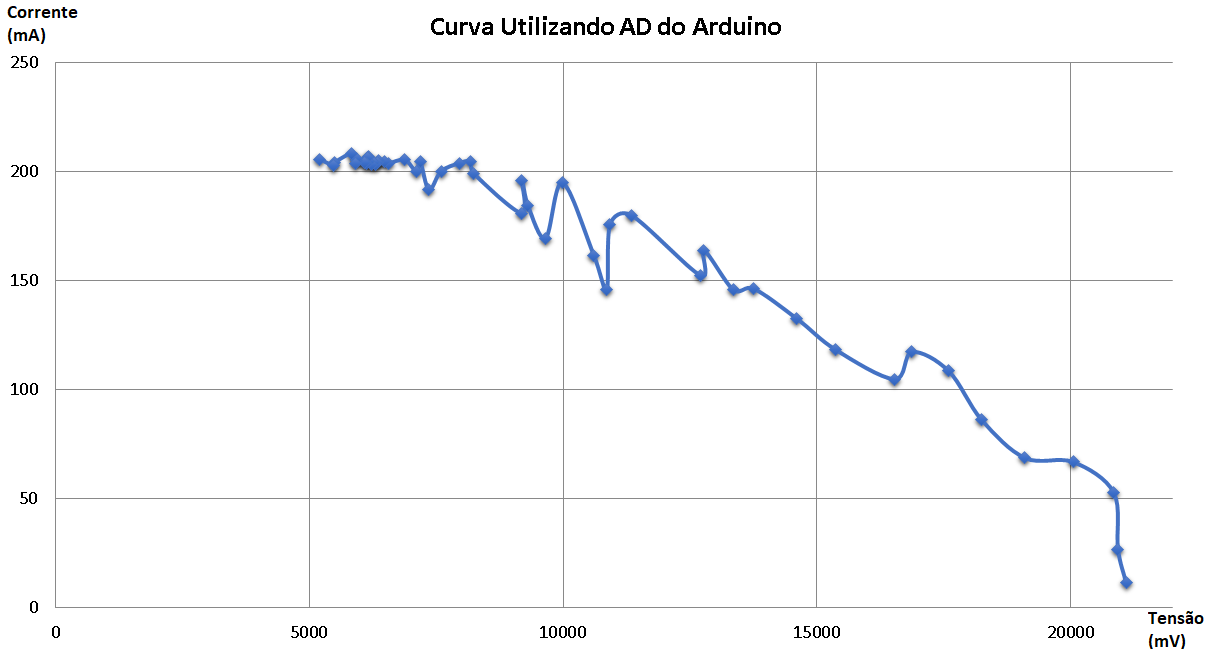
\includegraphics[scale=0.5]{imagens/CurvaArduino}
	\caption{Curva inicial utilizando o conversor AD interno do Arduino e um sinal de PWM com uma resolução de 255 pontos diferentes. Fonte: Elaborado pelo Autor. 	}
	\label{fig:CurvaArduino}
\end{figure}
\FloatBarrier

Após a coleta da curva referente a figura~\ref{fig:CurvaArduino} foi necessário a adaptação do circuito de maneira a gerar uma curva mais próxima à curva teórica do módulo fotovoltaico. Para isso houve o uso do sensor ADS1115, tendo como objetivo a diminuição do ruído em relação ao gerado pelo ADC do Arduino, além da possibilidade do uso de uma resolução de 16 bits, tendo assim uma maior sensibilidade no sensoriamento. Tendo como objetivo aumentar a quantidades de pontos para coleta e teste do circuito, houve a configuração de resolução do PWM Atmega328p de 8 bits para 14 bits, após configura o 16-bit \textit{Timer/Counter1} do microcontrolador, gerando o gráfico visto na figura \ref{fig:CurvaIVdeformadaII};

\FloatBarrier
\begin{figure}[!htbp]
	\centering
	%scale redimensiona a figura.
	%1.5 = 150% do tamanho original
	%1 = 100% do tamanho original
	%0.20 = 20% do tamanho original
	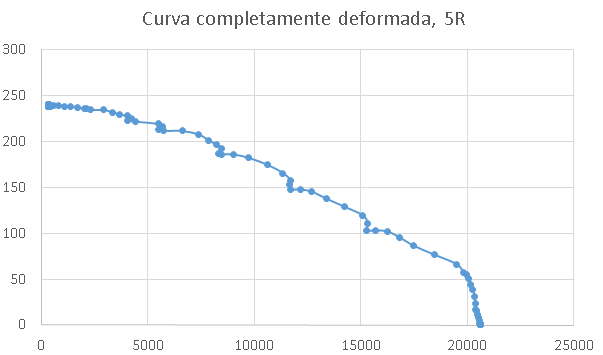
\includegraphics[scale=0.85]{imagens/CurvaIVdeformadaII}
	\caption{Curva IV deformada utilizando ADS1115 e  PWM com resolução de 14 bits . Fonte: Elaborado pelo Autor. 	}
	\label{fig:CurvaIVdeformadaII}
\end{figure}
\FloatBarrier

Após os testes foi possível observar a estabilidade do ADS1115 em relação ao ADC do Arduino. Tendo em consideração a curva da figura \ref{fig:CurvaIVdeformadaII}, houve a necessidade de alterar o circuito. Como mostrado por \citeauthorandyear{de2004manual}, há a necessidade de uma resistência com valor muito baixo em série com o painel para que se possa obter uma melhor curva IV, figura \ref{fig:CurvaResistencia}.
%Arrumar referencia
\FloatBarrier
\begin{figure}[!htbp]
	\centering
	%scale redimensiona a figura.
	%1.5 = 150% do tamanho original
	%1 = 100% do tamanho original
	%0.20 = 20% do tamanho original
	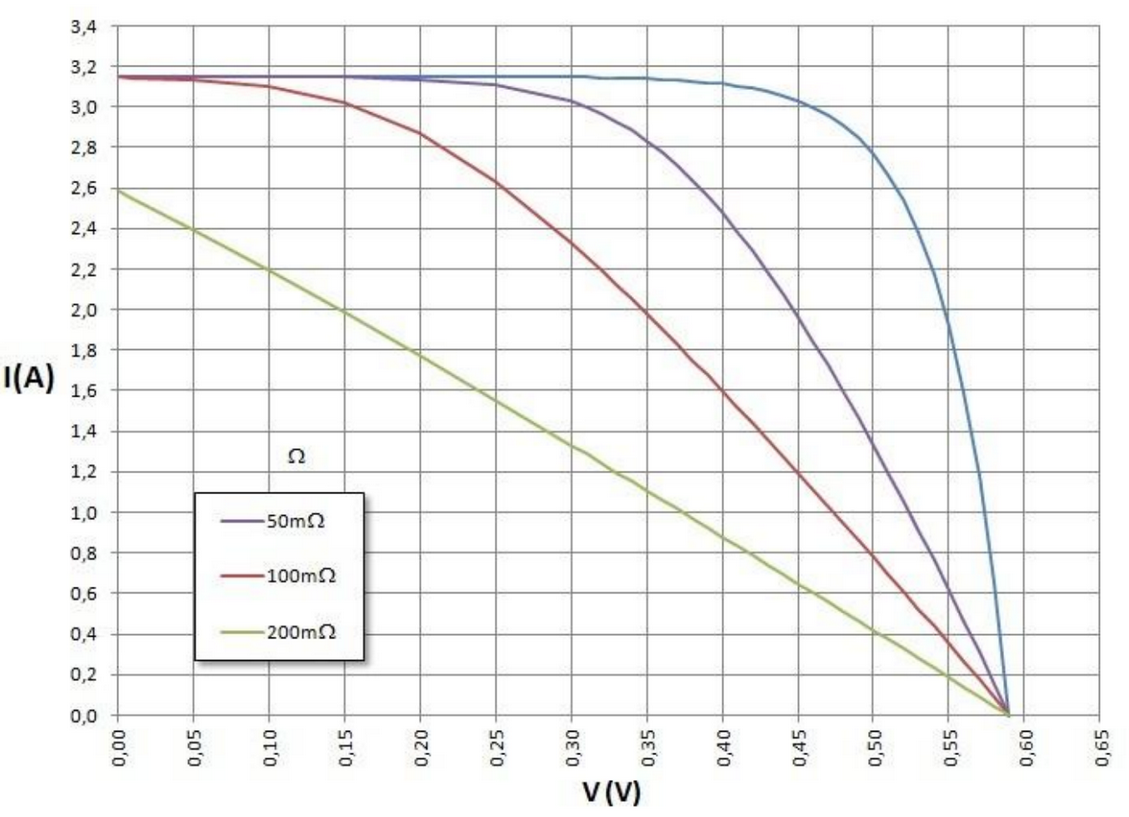
\includegraphics[scale=0.4]{imagens/CurvaResistencia}
	\caption{Curva IV com diferente resistências em série. Fonte: \cite{de2004manual}. 	}
	\label{fig:CurvaResistencia}
\end{figure}
\FloatBarrier

Tendo trocado os valores dos resistores e após retornar o sinal PWM para o padrão do Arduino foram feitos novos testes, figura~\ref{fig:Leitura}. A figura \ref{fig:Curvapoucos} mostra os resultados do novo teste.
\FloatBarrier
\begin{figure}[!htbp]
	\centering
	%scale redimensiona a figura.
	%1.5 = 150% do tamanho original
	%1 = 100% do tamanho original
	%0.20 = 20% do tamanho original
	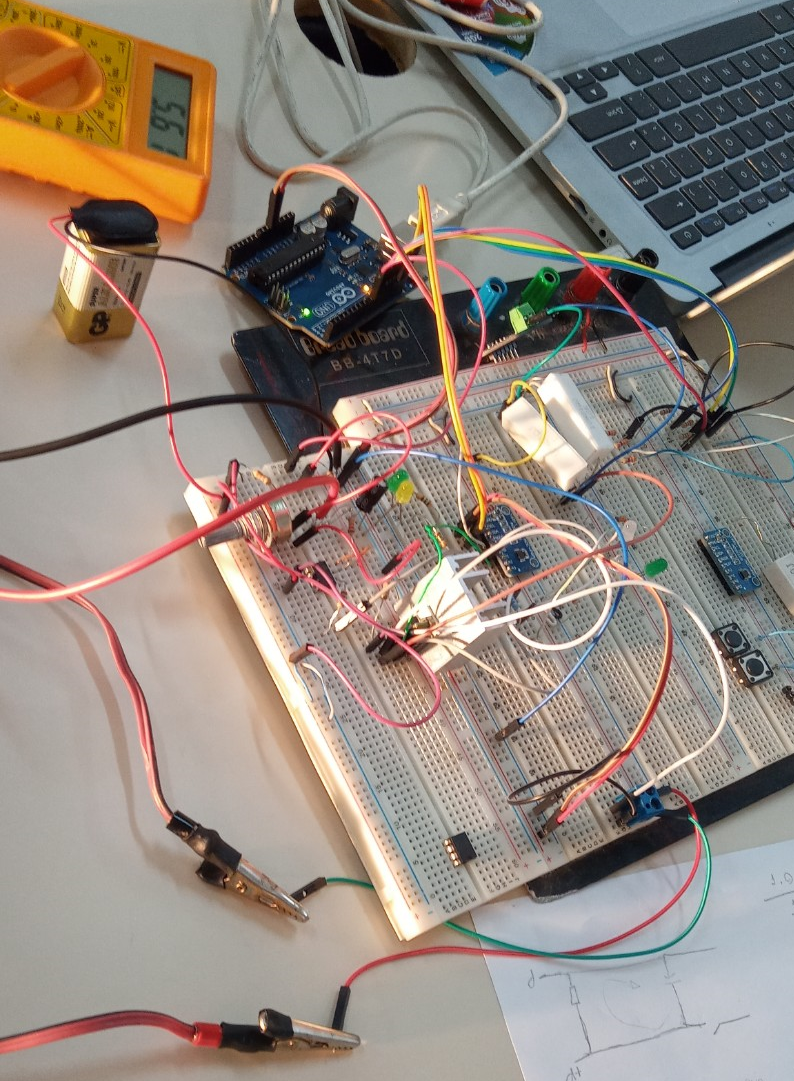
\includegraphics[scale=0.2]{imagens/Leitura.png}
	\caption{Imagem durante a leitura. Fonte: Elaborado pelo Autor. 	}
	\label{fig:Leitura}
\end{figure}
\FloatBarrier

\FloatBarrier
\begin{figure}[!htbp]
	\centering
	%scale redimensiona a figura.
	%1.5 = 150% do tamanho original
	%1 = 100% do tamanho original
	%0.20 = 20% do tamanho original
	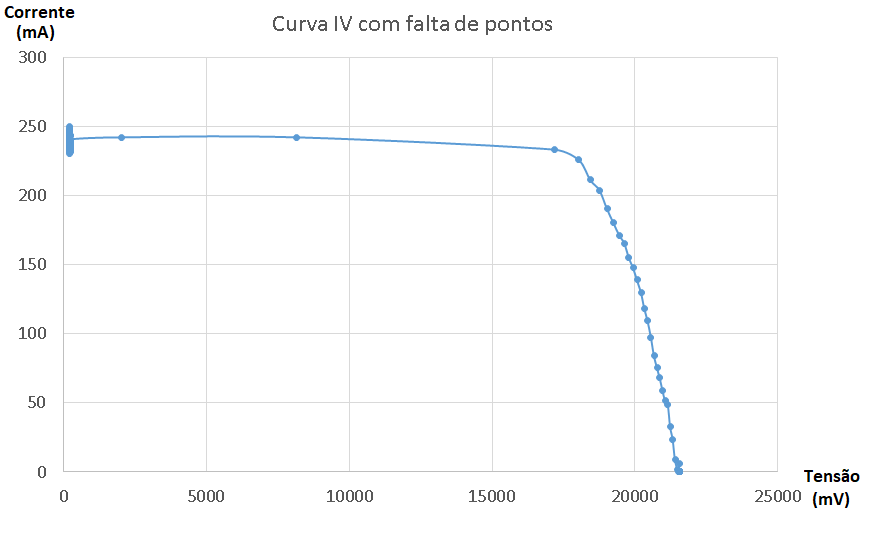
\includegraphics[scale=0.7]{imagens/CurvaIVpoucospontos}
	\caption{Curva IV com poucos pontos entre 5000 $mV$ e 15000 $mV$. Fonte: Elaborado pelo Autor. 	}
	\label{fig:Curvapoucos}
\end{figure}
\FloatBarrier

Após a troca do resistor de 3 Ohms para três resistores em paralelo, dois de 1 ohm e 1 resistor de 0,100 ohms, foi possível obter uma curva mais próxima da curva IV esperada, entretanto foi possível notar um grande acúmulo de pontos no início da curva e poucos pontos antes de $ 15000$ $mV$. Tendo como objetivo melhorar esse problema foi feito novamente o uso do PWM do Atmega328p configurado por fora da padrão do Arduino, como pode ser observado na figura \ref{fig:CurvaDeformada}.

\FloatBarrier
\begin{figure}[!htbp]
	\centering
	%scale redimensiona a figura.
	%1.5 = 150% do tamanho original
	%1 = 100% do tamanho original
	%0.20 = 20% do tamanho original
	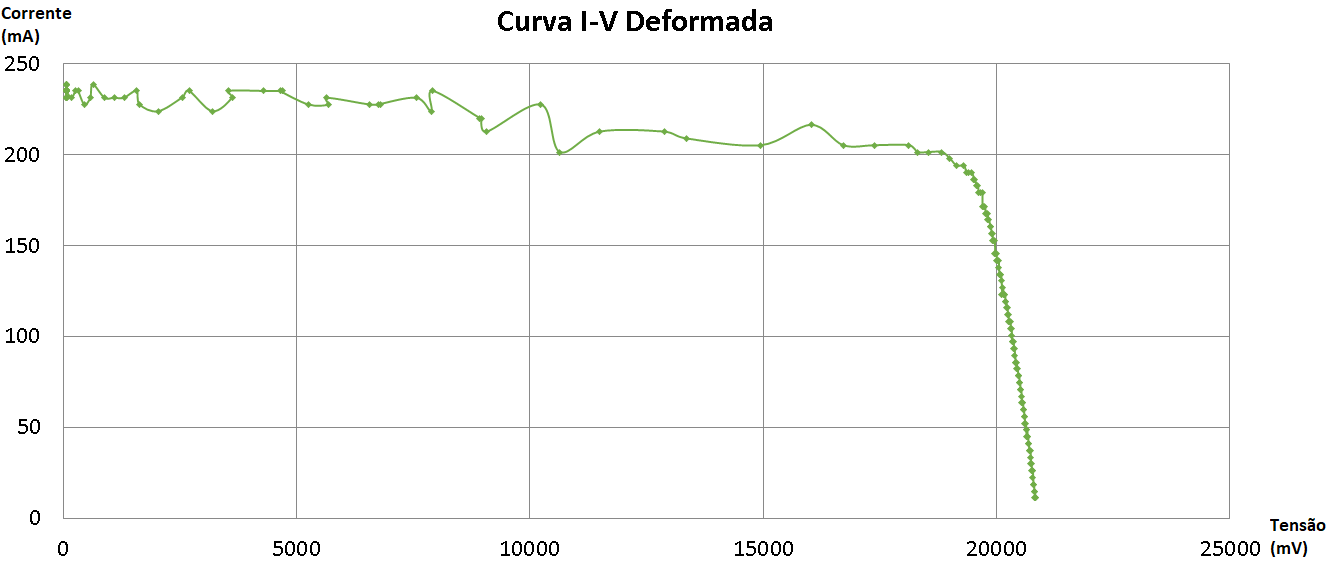
\includegraphics[scale=0.4]{imagens/CurvaIVdeformada}
	\caption{Curva IV deformada devido ao capacitor utilizado. Fonte: Elaborado pelo Autor. 	}
	\label{fig:CurvaDeformada}
\end{figure}
\FloatBarrier

Com uma resolução de PWM maior foi possível obter uma quantidade de pontos aceitável, entretanto houve a presença de uma variação nos valores coletados. Tendo esse problema em mente foram feitos testes utilizando capacitores no filtro utilizado no sinal PWM. Alterando o valor do capacitor de $10 uF$ para $100 uF$ e refeito o teste se deu o gráfico da figura \ref{fig:CurvaIVBoa}.

\FloatBarrier
\begin{figure}[!htbp]
	\centering
	%scale redimensiona a figura.
	%1.5 = 150% do tamanho original
	%1 = 100% do tamanho original
	%0.20 = 20% do tamanho original
	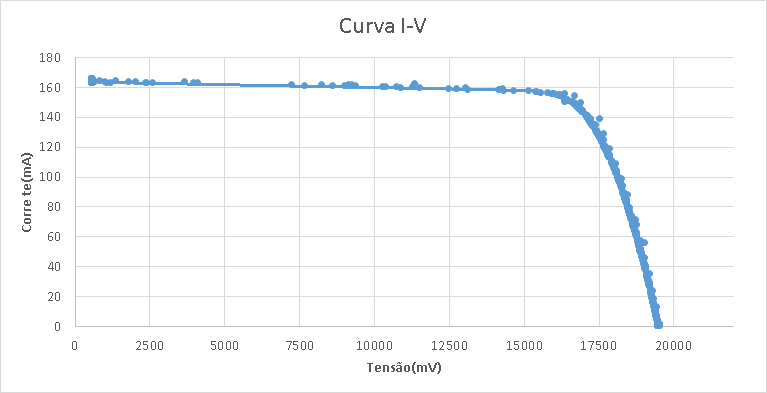
\includegraphics[scale=1.0]{imagens/CurvaIVfinal}
	\caption{Curva IV final. Fonte: Elaborado pelo Autor. 	}
	\label{fig:CurvaIVBoa}
\end{figure}
\FloatBarrier

%// Acrescentar Imagem de Curvas Morçadas e a foto do circuito na protoboard com o ADS ou ADC//

Após a alteração do circuito e da programação foi possível adquirir uma curva IV dentro do esperado, semelhante ao reportado na literatura, \citeauthorandyear{de2004manual}.
Considerando também os valores de irradiância dos testes da figura~\ref{fig:Icc} é possível observar que o valor de Corrente de Curto-circuito encontrado na figura~\ref{fig:CurvaIVBoa} está próximo do esperado.

\FloatBarrier
\begin{figure}[!htbp]
	\centering
	%scale redimensiona a figura.
	%1.5 = 150% do tamanho original
	%1 = 100% do tamanho original
	%0.20 = 20% do tamanho original
	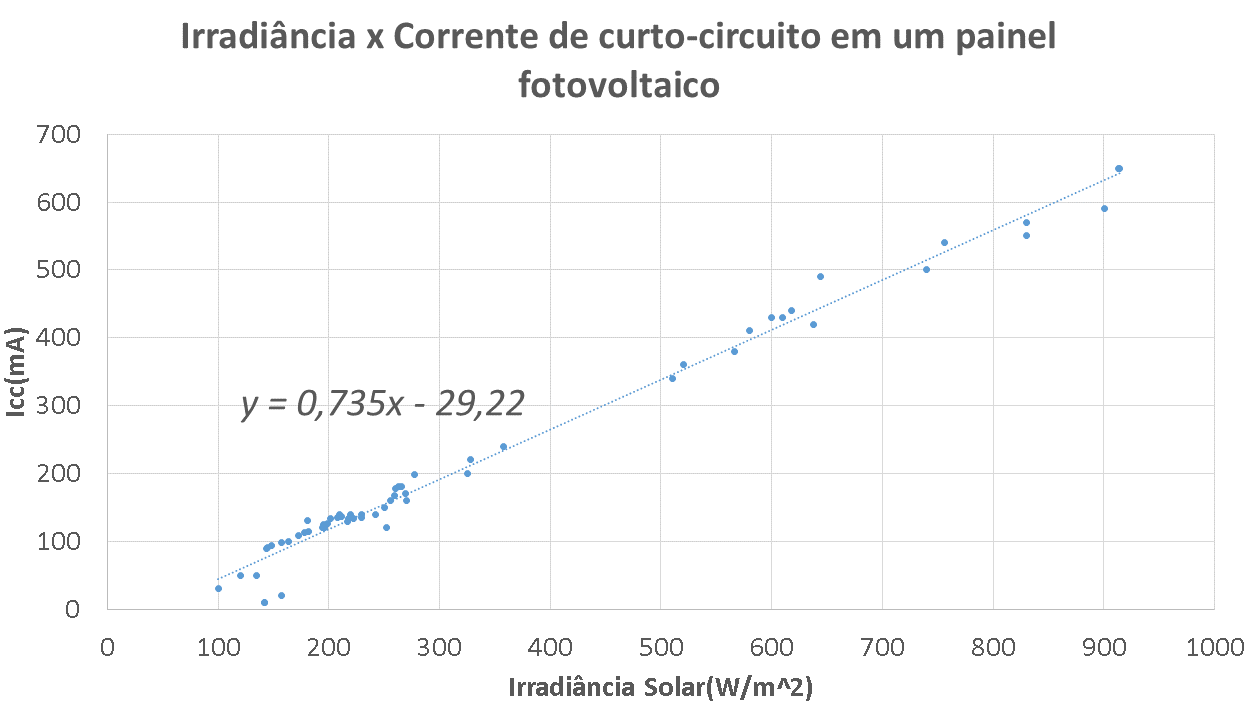
\includegraphics[scale=0.45]{imagens/Icc.png}
	\caption{Valores de Corrente de curto-circuito do painel em relação a irradiância. Fonte: Elaborado pelo Autor. 	}
	\label{fig:Icc}
\end{figure}
\FloatBarrier

A figura~\ref{fig:Icc} foi elabora em um teste durante uma pesquisa de iniciação cientifica no IFSP campus guarulhos. A pesquisa teve como objetivo observar se há relação entre os valores de irradiância solar e os valores de corrente de curto-circuito no painel fotovoltaico sobre influência dessa irradiância. Foram coletados valores de irradiância solar e da corrente de curto-circuito no mesmo instante, esse dados foram mesurados durante diferentes dias e horários. É possível observar a correlação desses valores ao se fazer um diagrama de dispersão como visto na figura~\ref{fig:Icc}. Utilizando a ferramenta Excel do pacote Office da Microsoft foi possível desenvolver o gráfico relacionando a irradiância solar com a corrente de curto-circuito da placa fotovoltaica, além da equação da reta de tendência.
Ao se observar a figura~\ref{fig:irrad} e ao se utilizar da equação da figura~\ref{fig:Icc}, observa-se que aos valores de corrente de curto-circuito dos testes inciais se encontra próximo do esperado.

\FloatBarrier
\begin{figure}[!htbp]
	\centering
	%scale redimensiona a figura.
	%1.5 = 150% do tamanho original
	%1 = 100% do tamanho original
	%0.20 = 20% do tamanho original
	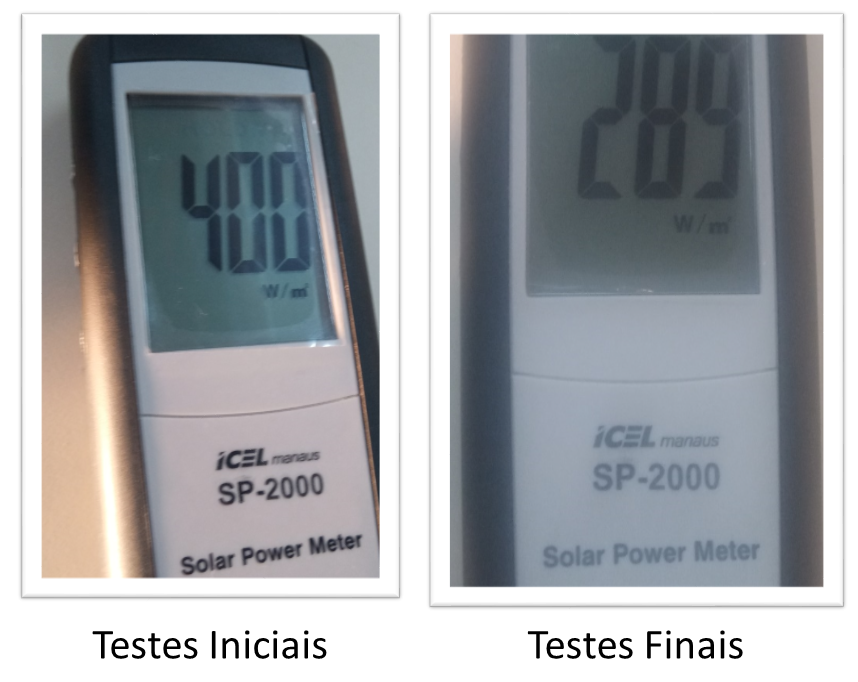
\includegraphics[scale=0.55]{imagens/irrad.png}
	\caption{Valor dado no solarímetro durante os testes iniciais e o teste final. Fonte: Elaborado pelo Autor. 	}
	\label{fig:irrad}
\end{figure}
\FloatBarrier

Tendo os valores de irradiância coletados através do solarímetro durantes os testes, como vistos na figura~\ref{fig:irrad}, é possível comparar os valores de corrente esperados, figura~\ref{fig:Iccs}, com os obtidos durante os testes.

\FloatBarrier
\begin{figure}[!htbp]
	\centering
	%scale redimensiona a figura.
	%1.5 = 150% do tamanho original
	%1 = 100% do tamanho original
	%0.20 = 20% do tamanho original
	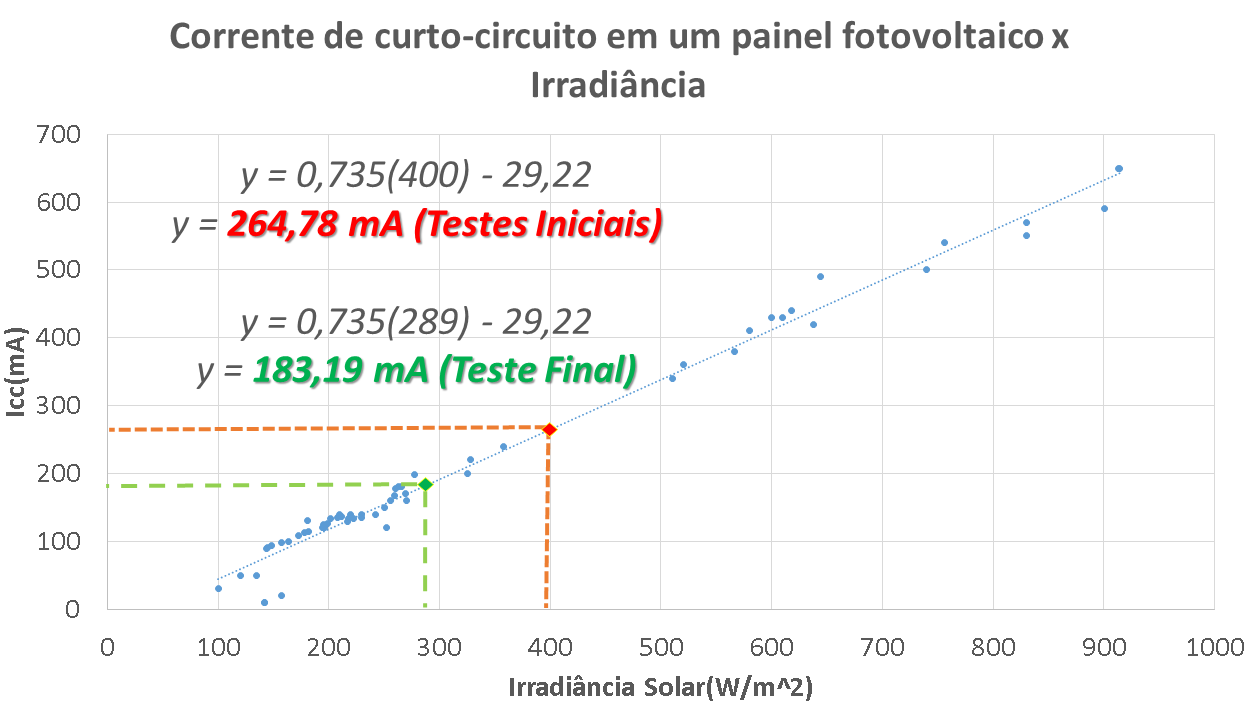
\includegraphics[scale=0.45]{imagens/Iccs.png}
	\caption{Valores de corrente esperados. Fonte: Elaborado pelo Autor. 	}
	\label{fig:Iccs}
\end{figure}
\FloatBarrier

\FloatBarrier
\begin{figure}[!htbp]
	\centering
	%scale redimensiona a figura.
	%1.5 = 150% do tamanho original
	%1 = 100% do tamanho original
	%0.20 = 20% do tamanho original
	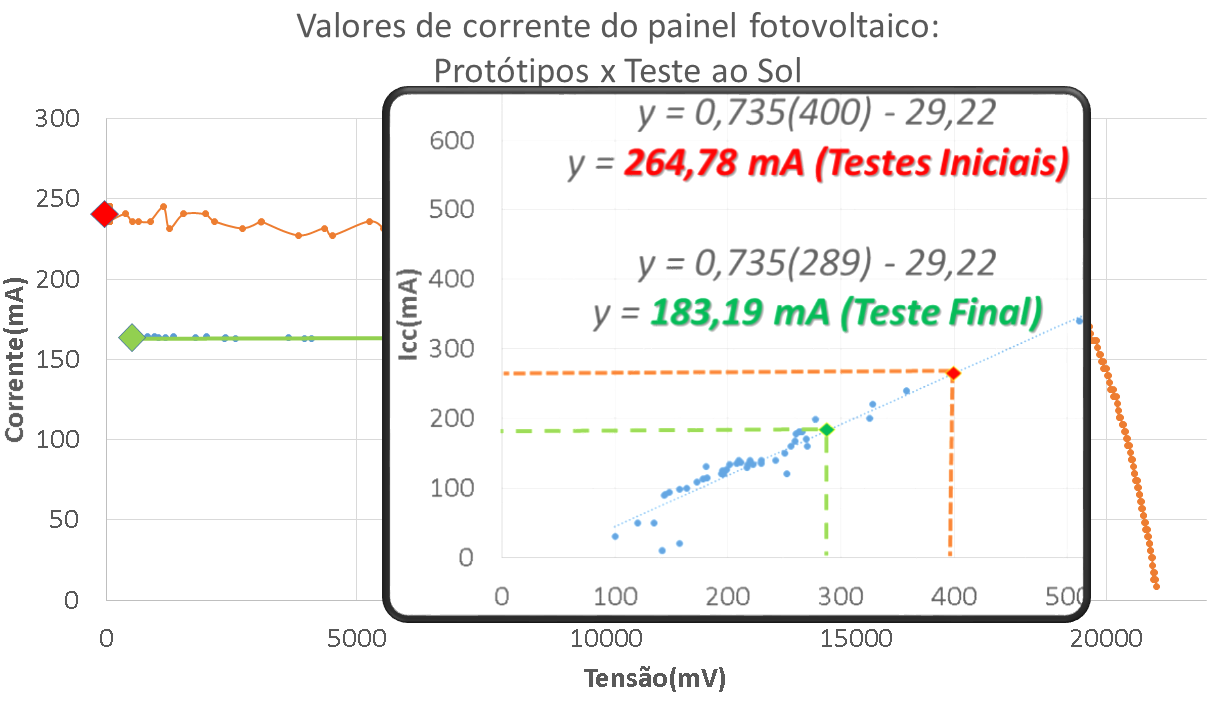
\includegraphics[scale=0.45]{imagens/IccIV.png}
	\caption{Valores de corrente quando comparado com os coletados pelo traçador. Fonte: Elaborado pelo Autor. 	}
	\label{fig:IccIV}
\end{figure}
\FloatBarrier

Pode-se observar na figura~\ref{fig:IccIV} que os valores obtidos pelo protótipo do traçador IV estão muito próximos dos valores esperados quando comparado com a figura~\ref{fig:Iccs}, estando entre $10$ e $20$ $mA$ abaixo do esperado.
\openany
%// Acrescentar fotos do Circuito na protoboard sendo testado (Tirar foto Logo menos), e acrescentar as curvas topzeras)

%Resultados Finais:
%Após concluir a fase de testes, iniciou-se a fase de confecção do circuito oficial, passando a configuração da \textit{protoboard} para uma placa de circuito impresso.... (Continua nos próximos episódios)  Texto dos resultados.